\documentclass[12pt,letterpapers]{IEEEtran}
\usepackage[utf8]{inputenc}
\usepackage[spanish]{babel}
\usepackage{amsmath}
\usepackage{amsfonts}
\usepackage{amssymb}
\usepackage{graphicx}
\usepackage{xcolor}
\usepackage{listings}
\usepackage{tikz}
\usepackage{float}
\date{today}

\title{Laboratorio 1: Microcontrolador Parte 1.}
\author{Alumnos: Felipe González Velázquez, Jonathan Chavarría Peña.}

\begin{document}
\renewcommand{\leftmark}{UNIVERSIDAD LATINA DE COSTA RICA -- BINGE-57 Arquitectura de Computadores}
\maketitle
	\begin{abstract}
En el  siguiente documento se describe  el proceso de implementación de una memoria RAM en la primera etapa de la arquitectura de un microcontolador. 
	\end{abstract}
\section{Descripción del sistema}
El sistema se compone de cinco entidades principales (\textbf{ROM}, \textbf{PC}, \textbf{ALU}, \textbf {FSM} y \textbf{RAM}) y los registros IR, AC, BC y W. Cada uno de estos sistemas es parte de una entidad general llamada \textbf{micro2}.

	\begin{figure}[H]
		\centering	
		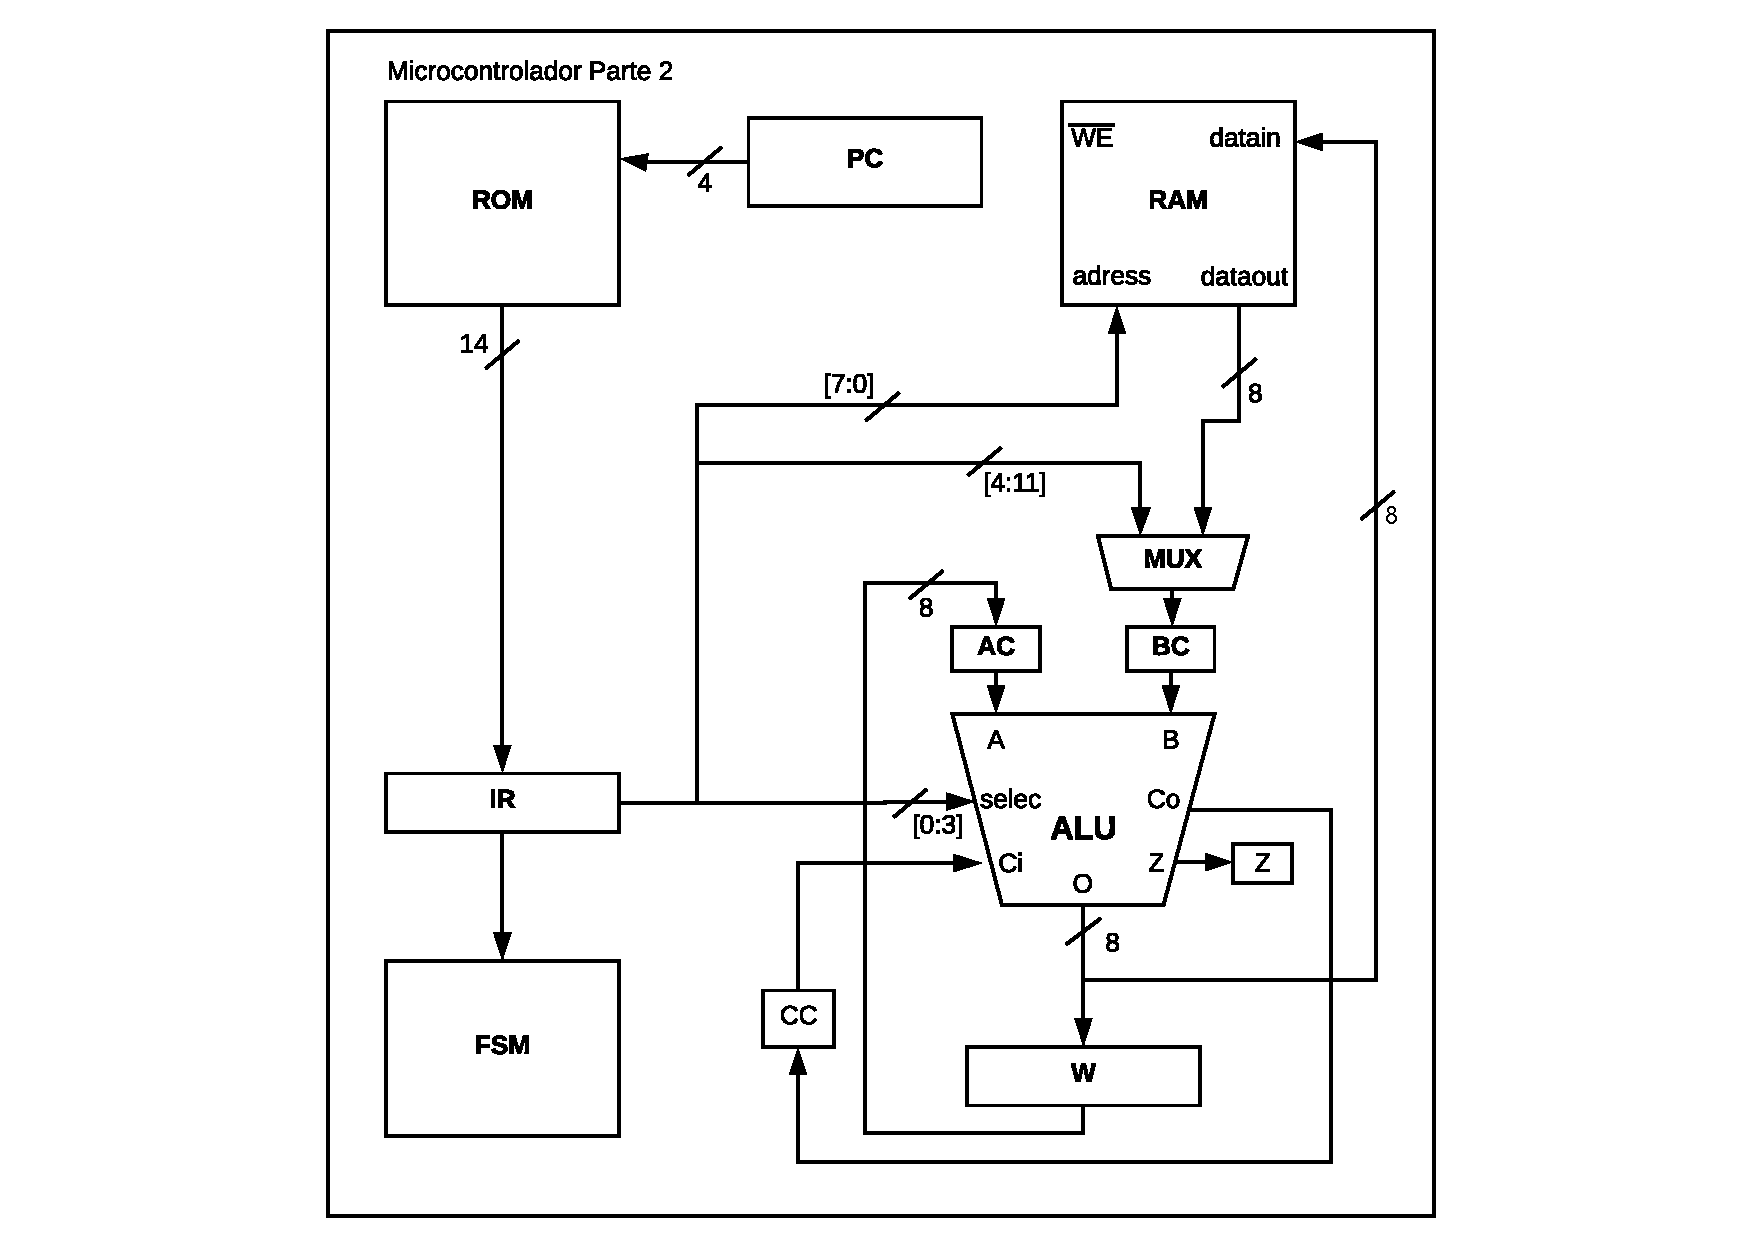
\includegraphics[width=0.5\textwidth]{graph} 
		\label{graph}
		\caption{Entidades principales del Sistema}
	\end{figure} 

El sistema es una continuación del laboratorio anterior por lo cual realiza las mismas funciones que antes, sin embargo, ahora posee funciones agregadas en cada estado.

\begin{figure}[H]
\centering
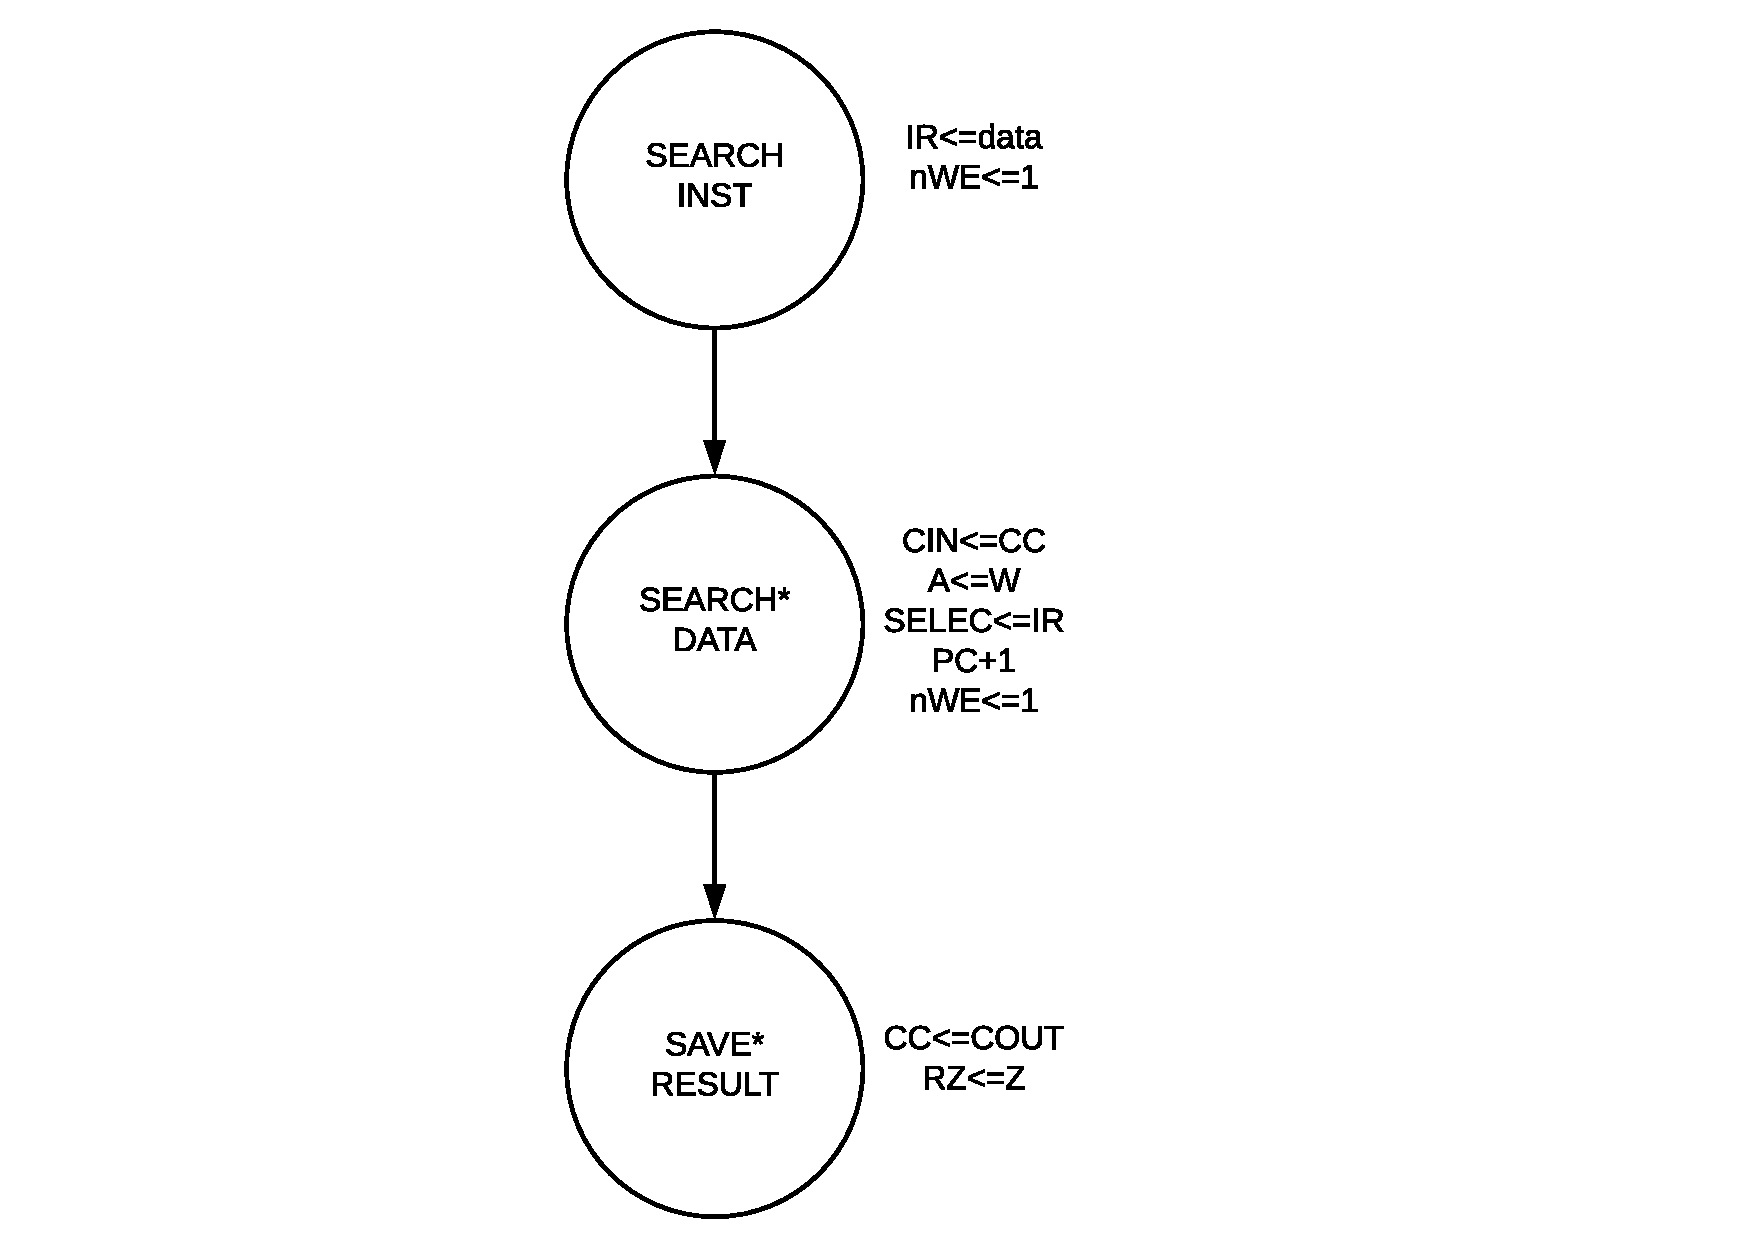
\includegraphics[scale=0.5]{graph2.pdf}
\caption{Diagrama de estados}
\end{figure}

\section{Listados del programa}

\section{Análisis De Resultados}

\section{Conceptos Aprendidos}  


\end{document}		